% =====================================================================
%  Rapport technique - Projet CI/CD avec Jenkins (ESGI Master 1)
%  Compiler avec pdflatex (Overleaf : compilateur pdfLaTeX).
%  Tout ce qui est en rouge = notes pour nous, à remplacer avant le rendu.
% =====================================================================
\documentclass[11pt,a4paper]{report}

% --- Langue et police ------------------------------------------------
\usepackage[utf8]{inputenc}
\usepackage[T1]{fontenc}
\usepackage[french]{babel}
\usepackage{lmodern}
\usepackage{csquotes}

% --- Mise en page ----------------------------------------------------
\usepackage[margin=2.5cm]{geometry}
\usepackage{fancyhdr}
\usepackage{titlesec}
\usepackage{enumitem}
\setlist{itemsep=2pt}
\setlength{\emergencystretch}{2em} % évite que le code dépasse dans la marge

% --- Tableaux, figures, code -----------------------------------------
\usepackage{graphicx}
\usepackage{booktabs}
\usepackage{tabularx}
\usepackage{float}
\usepackage{caption}
\usepackage{xcolor}
\usepackage{listings}
\usepackage[hidelinks]{hyperref}

\graphicspath{{images/}}

% Colonnes alignées à gauche (évite les grands espaces dans les cellules étroites)
\newcolumntype{L}[1]{>{\raggedright\arraybackslash}p{#1}}
\newcolumntype{Y}{>{\raggedright\arraybackslash}X}

% Chapitres sans la mention "Chapitre 1" sur une page entière
\titleformat{\chapter}{\normalfont\huge\bfseries}{\thechapter}{1em}{}
\titlespacing*{\chapter}{0pt}{0pt}{1.2em}

% En-tête et pied de page
\pagestyle{fancy}
\fancyhf{}
\fancyhead[L]{Projet CI/CD avec Jenkins}
\fancyhead[R]{\leftmark}
\fancyfoot[C]{\thepage}
\renewcommand{\headrulewidth}{0.4pt}
\fancypagestyle{plain}{\fancyhf{}\fancyfoot[C]{\thepage}\renewcommand{\headrulewidth}{0pt}}

% Code (Jenkinsfile, YAML, shell)
\definecolor{codebg}{gray}{0.96}
\lstset{
  basicstyle=\ttfamily\small,
  backgroundcolor=\color{codebg},
  frame=single, rulecolor=\color{gray!40},
  breaklines=true, columns=fullflexible,
  keepspaces=true, showstringspaces=false,
  literate={é}{{\'e}}1 {è}{{\`e}}1 {à}{{\`a}}1 {ç}{{\c c}}1 {ê}{{\^e}}1 {ô}{{\^o}}1
}

% Notes entre nous, en rouge (à virer avant le rendu)
\newcommand{\todo}[1]{\textcolor{red}{[#1]}}

% =====================================================================
\begin{document}

% ---------------------------------------------------------------------
%  Page de titre
% ---------------------------------------------------------------------
\begin{titlepage}
  \centering
  \vspace*{1cm}
  {\large ESGI \textendash{} Master 1 Architecture Logicielle\par}
  \vspace{0.5cm}
  {\large Module : CI/CD avec Jenkins\par}
  \vspace{3cm}
  {\Huge\bfseries Rapport technique\par}
  \vspace{0.6cm}
  {\LARGE Chaîne CI/CD complète sous Jenkins\par}
  \vspace{0.4cm}
  {\large Application : Job Application Tracker\par}
  \vspace{3cm}
  {\large\bfseries Équipe\par}
  \vspace{0.3cm}
  {\large
    Basma MORABIT \\
    Bastien LIEVRE \\
    Siham AIDROUS \\
    Mariam FATHALLAH \par}
  \vfill
  {\large Dépôt : \url{https://github.com/mariamfathallah/job-application-tracker}\par}
  \vspace{0.3cm}
  {\large 1\textsuperscript{er} novembre 2026\par}
\end{titlepage}

% ---------------------------------------------------------------------
%  Sommaire
% ---------------------------------------------------------------------
\tableofcontents
\clearpage

% =====================================================================
\chapter*{Introduction}
\addcontentsline{toc}{chapter}{Introduction}
% Contexte du projet, objectif, application choisie, plan du rapport.

\section*{Contexte et objectif}
Livrer souvent sans casser la production suppose d'automatiser tout ce qui se passe entre un commit et sa mise en ligne. C'est l'objet de ce projet, réalisé dans le cadre du module \emph{CI/CD avec Jenkins} : concevoir une chaîne d'intégration et de livraison continues complète sous Jenkins. Chaque commit y est construit, testé, analysé, empaqueté en un artefact versionné, puis livré en staging et, après validation humaine, en production.

L'enjeu n'est pas l'application elle-même, mais la chaîne qui l'entoure : elle doit être reproductible, rapide, fiable, et entièrement décrite dans le dépôt Git (\emph{Pipeline as Code}, configuration de Jenkins par code, environnements décrits par code).

\section*{L'application}
La chaîne est construite autour d'une application existante, \emph{Job Application Tracker}, qui permet de suivre ses candidatures tout au long d'un processus de recrutement. Elle se compose de trois parties :
\begin{itemize}
  \item une API REST en Java avec Spring Boot, sécurisée par JWT, organisée en couches (contrôleurs, services, dépôts) ;
  \item une interface web en React ;
  \item une base de données PostgreSQL, dont le schéma est géré par Liquibase.
\end{itemize}
Elle offre un terrain réaliste pour une chaîne CI/CD : deux langages à tester, une base de données pour les tests d'intégration, et une sonde de santé (Spring Boot Actuator) sur laquelle s'appuient les déploiements.

\section*{Périmètre réalisé}
L'équipe, composée de quatre membres, a réalisé la partie commune exigée et cinq modules, dont les deux de niveau 3 :
\begin{itemize}
  \item \textbf{partie commune} : outillage démarré en une commande (Jenkins, SonarQube, Nexus), builds exécutés sur un agent, job Multibranch déclenché par webhook, statut du build sur les pull requests, tests et Quality Gate bloquante, artefact versionné publié dans Nexus, déploiement automatique en staging puis en production après validation, Shared Library versionnée par tag, secrets dans les credentials Jenkins ;
  \item \textbf{Qualité et retour rapide} (niveau 1) ;
  \item \textbf{Releases automatisées} (niveau 1) ;
  \item \textbf{Déploiement blue/green} (niveau 2) ;
  \item \textbf{Environnements as Code} avec OpenTofu et Ansible (niveau 3) ;
  \item \textbf{Observabilité et métriques DORA} avec Prometheus et Grafana (niveau 3).
\end{itemize}

\section*{Plan du rapport}
Le chapitre~\ref{chap:architecture} présente l'architecture de la chaîne et le rôle de chaque composant. Le chapitre~\ref{chap:choix} justifie les choix techniques de chaque module et les alternatives écartées. Les chapitres~\ref{chap:pipeline} et~\ref{chap:deploiement} détaillent le pipeline puis les environnements et le déploiement. Le chapitre~\ref{chap:qualite} porte sur la qualité, et le chapitre~\ref{chap:dora} sur les métriques DORA mesurées pendant le projet. Les deux derniers chapitres reviennent sur les difficultés rencontrées et sur la répartition du travail.

% =====================================================================
\chapter{Architecture}\label{chap:architecture}
% Schéma de la chaîne, rôle de chaque composant.

\section{Vue d'ensemble}
La chaîne complète tient dans le dépôt Git : un push déclenche le pipeline, qui construit, vérifie, publie puis déploie l'application dans deux environnements, pendant que Prometheus et Grafana mesurent l'ensemble.

\begin{lstlisting}[caption={Architecture de la chaîne CI/CD}]
 git push / PR --> GitHub --> webhook (smee) --> Jenkins controller (0 executor)
                                                        |
                                                        v
                   agent-1 : JDK 21, Node 22, Docker, OpenTofu, Ansible
   commit lint (PR) -> lint + tests -> SonarQube + Quality Gate || tests d'integration
   -> release (tag vX.Y.Z) -> jar X.Y.Z-<hash> -> Nexus
   -> plan OpenTofu -> staging (auto) -> validation manuelle -> production

   staging / production : reseau Docker + PostgreSQL + proxy nginx + blue/green
   Prometheus <-- Jenkins, staging, production, exporter DORA --> Grafana
\end{lstlisting}

% \begin{figure}[H]
%   \centering
%   \includegraphics[width=\textwidth]{architecture.png}
%   \caption{Architecture de la chaîne CI/CD}
% \end{figure}

\section{Rôle de chaque composant}
\begin{table}[H]
  \centering
  \begin{tabularx}{\textwidth}{@{}lY@{}}
    \toprule
    \textbf{Composant} & \textbf{Rôle} \\
    \midrule
    Jenkins (controller) & orchestre les builds, ne build jamais lui-même (0 executor) \\
    Agent \texttt{agent-1} & exécute tous les builds (JDK, Node, Docker, OpenTofu, Ansible) \\
    SonarQube & analyse le code, Quality Gate bloquante \\
    Nexus & stocke les jar versionnés \\
    smee & relaie les webhooks GitHub vers notre Jenkins local \\
    Staging / Production & environnements où tourne l'application (ports 8082 et 8083) \\
    Prometheus / Grafana & collecte et affichage des métriques \\
    \bottomrule
  \end{tabularx}
  \caption{Composants de la plateforme}
\end{table}

\section{Démarrage en une commande}
Toute la plateforme est décrite dans un seul fichier, \texttt{ci/docker-compose.yml}, et démarre avec \texttt{docker compose up -d --build}. Rien n'est configuré à la main dans les interfaces : un membre de l'équipe, ou un correcteur, obtient la même plateforme à partir du dépôt et d'un fichier \texttt{ci/.env}.

\begin{itemize}
  \item \textbf{Jenkins} est construit avec sa liste de plugins (\texttt{ci/jenkins/plugins.txt}) et configuré par \textbf{JCasC} (\texttt{ci/jenkins/casc.yaml}) : utilisateur administrateur, agent, credentials, Shared Library et job Multibranch sont créés au démarrage. Les secrets viennent des variables de \texttt{ci/.env}, jamais du dépôt.
  \item \textbf{L'agent} est une image dédiée (JDK 21, Node 22, client Docker, OpenTofu 1.10.6, Ansible), qui se connecte seule au controller. Il utilise le Docker de l'hôte (\emph{docker-out-of-docker}) : son workspace est monté au même chemin (\texttt{/opt/jenkins-agent}) côté hôte et côté agent, pour que les conteneurs lancés par les builds voient les mêmes fichiers.
  \item \textbf{Volumes} : les caches Maven et npm accélèrent les builds, et l'état OpenTofu (\texttt{tf\_state}) survit aux redémarrages.
  \item \textbf{Initialisation} : deux scripts idempotents complètent ce que Docker ne peut pas faire seul, la création du dépôt d'artefacts dans Nexus (\texttt{bootstrap-nexus.sh}) et le webhook SonarQube vers Jenkins (\texttt{bootstrap-sonar.sh}).
\end{itemize}

Tout étant décrit par code, chaque changement de la plateforme passe par une pull request relue, et la procédure complète de remise en route est donnée dans le \texttt{README.md} du dépôt.

% =====================================================================
\chapter{Choix techniques et justifications}\label{chap:choix}
% Par module, avec les alternatives écartées.

\section{Partie commune}
Le job Multibranch utilise la source \textbf{GitHub} (\emph{GitHub Branch Source}), déclarée dans \texttt{ci/jenkins/casc.yaml}. Jenkins découvre ainsi les branches et les pull requests (builds \texttt{PR-<n>}) et publie le résultat de chaque build sur la PR. Jenkins tournant en local, il n'est pas joignable depuis Internet : le webhook GitHub passe par un relais \textbf{smee.io}, exécuté dans le conteneur \texttt{ci-smee} de la stack.

\begin{table}[H]
  \centering
  \small
  \begin{tabularx}{\textwidth}{@{}L{3cm}L{3cm}Y@{}}
    \toprule
    \textbf{Choix} & \textbf{Alternative écartée} & \textbf{Raison} \\
    \midrule
    Source GitHub & Source Git simple & la source Git ne voit pas les pull requests et ne publie pas de statut \\
    \addlinespace
    smee.io dans un conteneur & ngrok, Tailscale & vu en TP, aucun compte ni ouverture réseau ; le relais démarre avec le reste de la stack, sans terminal à laisser ouvert \\
    \addlinespace
    Un Jenkins de référence (token en écriture) & Chaque membre publie ses statuts & quatre Jenkins écrivant le même check rendraient le statut ambigu ; les autres membres utilisent un token en lecture seule \\
    \bottomrule
  \end{tabularx}
  \caption{Choix de l'intégration GitHub}
\end{table}

\textbf{Shared Library.} Les étapes communes (publication dans Nexus, déploiement, notification) sont regroupées dans un dépôt séparé, \texttt{jenkins-shared-library}, plutôt que copiées dans le Jenkinsfile. Une correction se fait ainsi à un seul endroit. La bibliothèque est déclarée par code dans \texttt{casc.yaml} et chargée par \texttt{@Library('jenkins-shared-library@v1.2.0')}. Une bibliothèque globale s'exécute hors sandbox, avec une confiance totale : on l'épingle donc sur un tag, pour que modifier sa branche principale ne change aucun pipeline.

\section{Qualité et retour rapide}
\begin{table}[H]
  \centering
  \small
  \begin{tabularx}{\textwidth}{@{}L{2.6cm}L{3cm}L{2.8cm}Y@{}}
    \toprule
    \textbf{Besoin} & \textbf{Choix} & \textbf{Alternative écartée} & \textbf{Raison} \\
    \midrule
    Mesurer la couverture & JaCoCo & Cobertura & intégré à Maven, lu par Jenkins et SonarQube \\
    \addlinespace
    Imposer un minimum & règle \texttt{check} de JaCoCo & contrôle manuel & le build échoue automatiquement sous le seuil \\
    \addlinespace
    Publier les rapports & plugins JUnit et Coverage & lecture des fichiers à la main & résultats visibles sur la page du build \\
    \addlinespace
    Notifier & webhook Discord & e-mail, Slack & une simple URL, aucun plugin \\
    \addlinespace
    Aller vite & parallélisme, caches Maven et npm & exécution en séquence & caches montés en volumes sur l'agent \\
    \bottomrule
  \end{tabularx}
  \caption{Choix techniques du module Qualité}
\end{table}

\section{Releases automatisées}
Les messages de commit suivent la convention \emph{Conventional Commits}, vérifiée par \textbf{commitlint} dès la première étape du pipeline, sur les pull requests : un message invalide fait échouer le build immédiatement. Une fois tous les contrôles passés, \textbf{semantic-release} analyse les commits depuis le dernier tag et en déduit la version : \texttt{fix} et \texttt{perf} donnent un correctif, \texttt{feat} une version mineure, \texttt{BREAKING CHANGE} une version majeure. Il génère le changelog, crée le tag \texttt{vX.Y.Z} et publie une GitHub Release avec les notes de version. L'artefact publié dans Nexus est nommé \texttt{X.Y.Z-<hash>} : version issue du tag et hash du commit.

L'étape \emph{Release} ne s'exécute que sur \texttt{main}, après les tests, la Quality Gate et les tests d'intégration : seul du code validé reçoit un numéro de version. Elle est de plus réservée au Jenkins de référence (\texttt{RELEASES\_ENABLED=true}), pour qu'un seul Jenkins crée les tags.

\begin{table}[H]
  \centering
  \small
  \begin{tabularx}{\textwidth}{@{}L{3cm}L{3cm}Y@{}}
    \toprule
    \textbf{Choix} & \textbf{Alternative écartée} & \textbf{Raison} \\
    \midrule
    semantic-release & release-please & release-please fonctionne par \og PR de release \fg{} et est pensé pour GitHub Actions ; semantic-release s'exécute en une commande dans le pipeline \\
    \addlinespace
    Vérification en CI & Hook Git local (husky) & un hook local peut être contourné ; la CI s'applique à tous \\
    \addlinespace
    Pas de commit du \texttt{CHANGELOG.md} & Plugin \texttt{@semantic-\allowbreak release/\allowbreak git} & le commit relancerait un build et serait bloqué par la protection de \texttt{main} ; le changelog est archivé dans Jenkins et figure dans la GitHub Release \\
    \addlinespace
    Commentaires automatiques désactivés & Comportement par défaut & la première release couvre tout l'historique : le plugin aurait commenté toutes les anciennes PR du dépôt \\
    \bottomrule
  \end{tabularx}
  \caption{Choix du module Releases automatisées}
\end{table}

Pendant le projet, neuf versions ont été calculées et publiées automatiquement :

\begin{table}[H]
  \centering
  \small
  \begin{tabular}{@{}llll@{}}
    \toprule
    \textbf{Version} & \textbf{PR} & \textbf{Type du commit} & \textbf{Effet} \\
    \midrule
    v1.0.0 & \#12 & \texttt{docs} & première release, calculée sur tout l'historique \\
    v1.1.0 & \#13 & \texttt{feat} & version mineure \\
    v1.1.1 & \#14 & \texttt{perf} & correctif \\
    v1.1.2 & \#16 & \texttt{fix} & correctif \\
    v1.2.0 & \#15 & \texttt{feat} & version mineure \\
    v1.2.1 & \#17 & \texttt{perf} & correctif \\
    v1.3.0 & \#18 & \texttt{feat} & version mineure \\
    v1.3.1 & \#19 & \texttt{fix} & correctif \\
    v1.4.0 & \#23 & \texttt{feat} & version mineure \\
    \bottomrule
  \end{tabular}
  \caption{Versions publiées par semantic-release}
\end{table}

Les commits \texttt{ci}, \texttt{docs} et \texttt{chore} suivants (\#21, \#22, \#24, \#25) n'ont pas produit de version : ils ne modifient pas le livrable.

\begin{figure}[H]
  \centering
  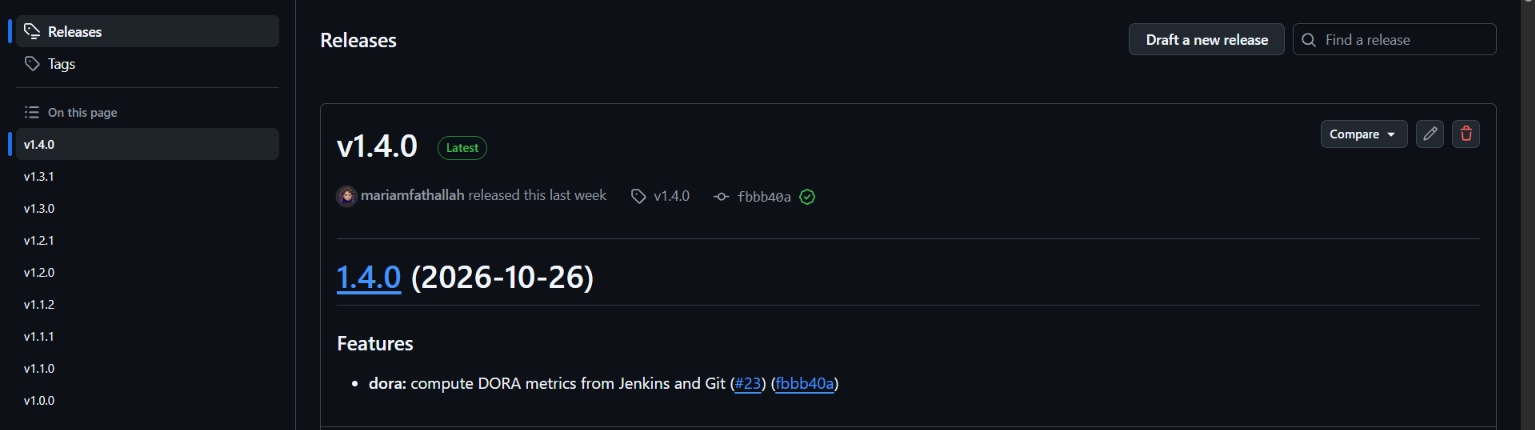
\includegraphics[width=0.85\textwidth]{releases.png}
  \caption{Versions publiées automatiquement par semantic-release}
\end{figure}

\section{Blue/green}
Chaque environnement comporte un proxy \textbf{nginx}, seul port publié, et deux conteneurs applicatifs \texttt{blue} et \texttt{green} sans port publié. La nouvelle version est toujours déployée sur la couleur inactive, vérifiée, puis le proxy bascule. Le déroulé complet et le retour arrière sont décrits en section~\ref{sec:bluegreen}.

\begin{table}[H]
  \centering
  \small
  \begin{tabularx}{\textwidth}{@{}L{3cm}L{3cm}Y@{}}
    \toprule
    \textbf{Choix} & \textbf{Alternative écartée} & \textbf{Raison} \\
    \midrule
    nginx & Traefik & configuration simple et lisible ; bascule par rechargement, sans coupure \\
    \addlinespace
    Proxy géré par Ansible & Proxy décrit dans OpenTofu & nginx refuse de démarrer si sa cible n'existe pas encore : l'ordre \og application puis proxy \fg{} se gère naturellement dans un playbook ; OpenTofu reste consacré à l'infrastructure durable \\
    \addlinespace
    Blue/green en staging et en production & Production seule & staging doit être une copie fidèle de la production ; la stratégie est testée à chaque déploiement \\
    \addlinespace
    Couleur active mémorisée dans le proxy & Fichier sur l'agent & l'agent n'est pas persistant ; le proxy est la source de vérité du trafic \\
    \bottomrule
  \end{tabularx}
  \caption{Choix du module Blue/green}
\end{table}

\section{Environnements as Code}
\begin{table}[H]
  \centering
  \small
  \begin{tabularx}{\textwidth}{@{}L{3cm}L{3cm}Y@{}}
    \toprule
    \textbf{Choix} & \textbf{Alternative écartée} & \textbf{Raison} \\
    \midrule
    OpenTofu & Terraform & même langage et mêmes providers, mais licence libre (MPL) ; Terraform est passé sous licence BSL \\
    \addlinespace
    Provider Docker (\texttt{kreuzwerker/\allowbreak docker}) & Machines virtuelles dans un cloud & aucun compte ni coût, environnements recréables sur chaque poste ; passer au cloud reviendrait à changer de provider, la structure restant la même \\
    \addlinespace
    OpenTofu pour l'infrastructure, Ansible pour l'application & Un seul outil pour tout & l'infrastructure (réseau, base, secrets) change rarement ; l'application change à chaque livraison, ce qui relève de la configuration \\
    \addlinespace
    Plan enregistré puis appliqué tel quel & \texttt{tofu apply} direct & ce qui a été relu est exactement ce qui est appliqué ; si l'infrastructure a changé entre-temps, OpenTofu refuse le plan périmé \\
    \addlinespace
    État dans un volume Docker de l'agent & État dans Git & l'état contient les mots de passe générés : il ne doit jamais être versionné \\
    \addlinespace
    Secrets générés (\texttt{random\_\allowbreak password}) & Secrets écrits dans des fichiers & aucun secret à créer ni à partager ; chaque environnement a les siens \\
    \bottomrule
  \end{tabularx}
  \caption{Choix du module Environnements as Code}
\end{table}

\section{Observabilité et DORA}
Le principe directeur : la mesure doit être automatique, reproductible et lancée avec le reste de l'outillage par un seul \texttt{docker compose up -d}.

\begin{table}[H]
  \centering
  \small
  \begin{tabularx}{\textwidth}{@{}L{2.5cm}L{2.9cm}L{2.9cm}Y@{}}
    \toprule
    \textbf{Besoin} & \textbf{Choix} & \textbf{Alternative écartée} & \textbf{Raison} \\
    \midrule
    Collecter et stocker les métriques & Prometheus, rétention 180 jours & Envoi depuis le pipeline (Pushgateway) & Prometheus va chercher les métriques lui-même : un build qui plante n'empêche pas la mesure \\
    \addlinespace
    Afficher les tableaux de bord & Grafana configuré par fichiers & Tableaux de bord créés à la main & Versionnés dans Git, identiques sur chaque poste et relus en PR \\
    \addlinespace
    Métriques de Jenkins & Plugin \texttt{prometheus} & Aucune & Standard, une ligne dans \texttt{plugins.txt} \\
    \addlinespace
    Métriques de l'application & Micrometer (\texttt{/actuator/\allowbreak prometheus}) & Agent JMX & Déjà intégré à Spring Boot via Actuator \\
    \addlinespace
    Calcul des métriques DORA & Exporter maison en Python & Plugins DORA, outils externes (Four Keys\ldots) & Aucun plugin ne gère nos règles (validation manuelle, retour arrière blue/green, deux branches) ; les outils externes demandent un service hébergé \\
    \bottomrule
  \end{tabularx}
  \caption{Choix techniques du module Observabilité et DORA}
\end{table}

L'exporter n'utilise que la bibliothèque standard de Python, sans dépendance à installer. Il est couvert par 14 tests, dont un test de bout en bout contre un faux Jenkins.

% =====================================================================
\chapter{Pipeline détaillé}\label{chap:pipeline}
% Étapes, Shared Library, secrets.

\section{Les étapes du Jenkinsfile}
\begin{table}[H]
  \centering
  \small
  \begin{tabularx}{\textwidth}{@{}L{3.6cm}L{2.6cm}Y@{}}
    \toprule
    \textbf{Étape} & \textbf{Quand} & \textbf{Rôle} \\
    \midrule
    Commit lint & pull request & messages au format Conventional Commits \\
    Lint \& tests & toujours & backend et frontend en parallèle \\
    Analyse \& intégration & toujours & SonarQube et tests d'intégration en parallèle \\
    Release & \texttt{main} & version, tag, changelog \\
    Package \& publish & toujours & artefact publié dans Nexus \\
    Infra plan & toujours & plan OpenTofu \\
    Publish plan on PR & pull request & plan publié en commentaire \\
    Deploy staging & \texttt{main} & déploiement automatique \\
    Deploy production & \texttt{main} & validation manuelle, puis déploiement \\
    \bottomrule
  \end{tabularx}
  \caption{Étapes du pipeline}
\end{table}

L'étape de mise en production montre comment le pipeline combine validation humaine, infrastructure et déploiement :

\begin{figure}[H]
  \centering
  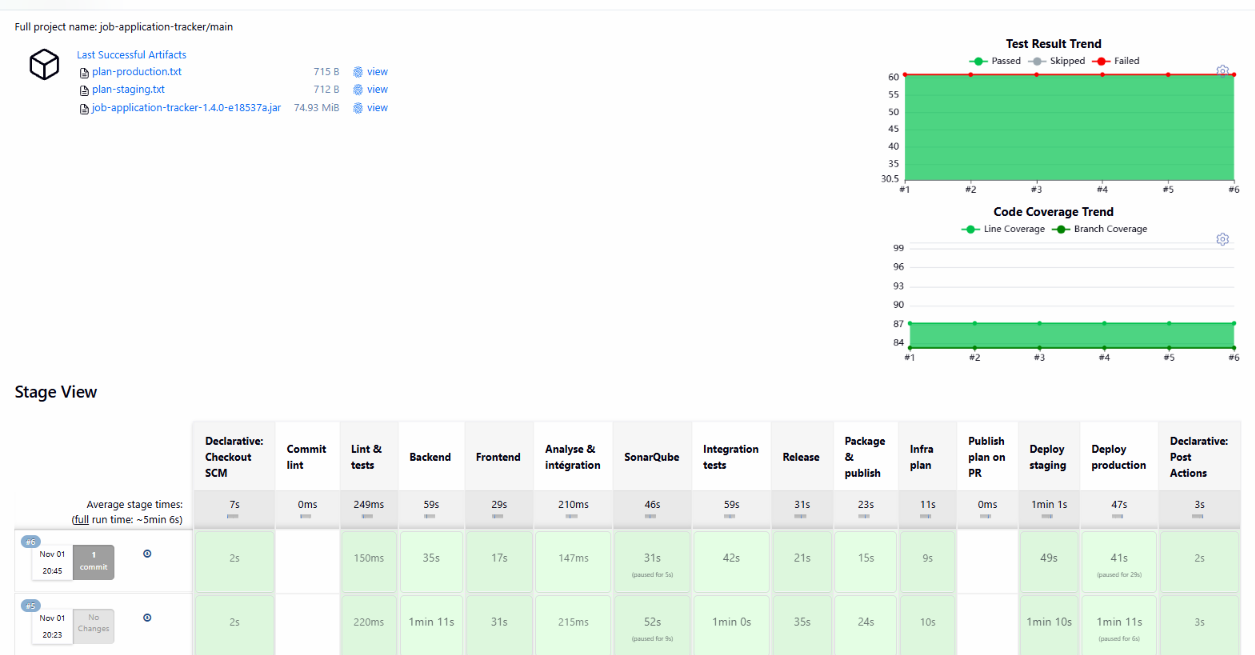
\includegraphics[width=\textwidth]{pipeline-main.png}
  \caption{Builds de \texttt{main} : toutes les étapes, jusqu'à la production}
\end{figure}

\begin{lstlisting}[caption={Étape \emph{Deploy production} du Jenkinsfile}]
stage('Deploy production') {
  when { expression { env.BRANCH_NAME == env.DEPLOY_BRANCH } }
  steps {
    timeout(time: 30, unit: 'MINUTES') {
      input message: "Déployer ${env.VERSION} en production ? (plan d'infra : artefact plan-production.txt)", submitter: 'admin'
    }
    sh 'sh ci/scripts/infra.sh apply production'   // applique exactement le plan validé
    deployTo('production')
  }
}
\end{lstlisting}

\begin{itemize}
  \item \texttt{when} : seule la branche de déploiement (\texttt{main}) va jusqu'en production ;
  \item \texttt{input} avec \texttt{submitter} : seul l'utilisateur \texttt{admin} peut valider, en voyant la version et le plan d'infrastructure ; sans réponse sous 30 minutes, le build s'arrête sans déployer ;
  \item \texttt{infra.sh apply} applique le plan calculé plus tôt dans le même build, celui qui a été relu ;
  \item \texttt{deployTo} vient de la Shared Library et lance le déploiement blue/green.
\end{itemize}

\section{Déclenchement}
Un push sur GitHub déclenche un webhook, relayé par smee jusqu'à Jenkins (\texttt{/github-webhook/}) : le build démarre en environ deux secondes. Un scan du dépôt toutes les heures reste en place en secours, si un événement est perdu.

Sur une pull request, Jenkins construit le résultat de la fusion avec \texttt{main} et publie le statut du build sur la PR. La branche \texttt{main} est protégée :
\begin{itemize}
  \item toute modification passe par une pull request ;
  \item une approbation d'un autre membre est obligatoire ;
  \item le check Jenkins doit être vert ;
  \item la fusion se fait uniquement en \emph{squash}, ce qui garde un commit par PR et un historique propre pour semantic-release.
\end{itemize}

\begin{figure}[H]
  \centering
  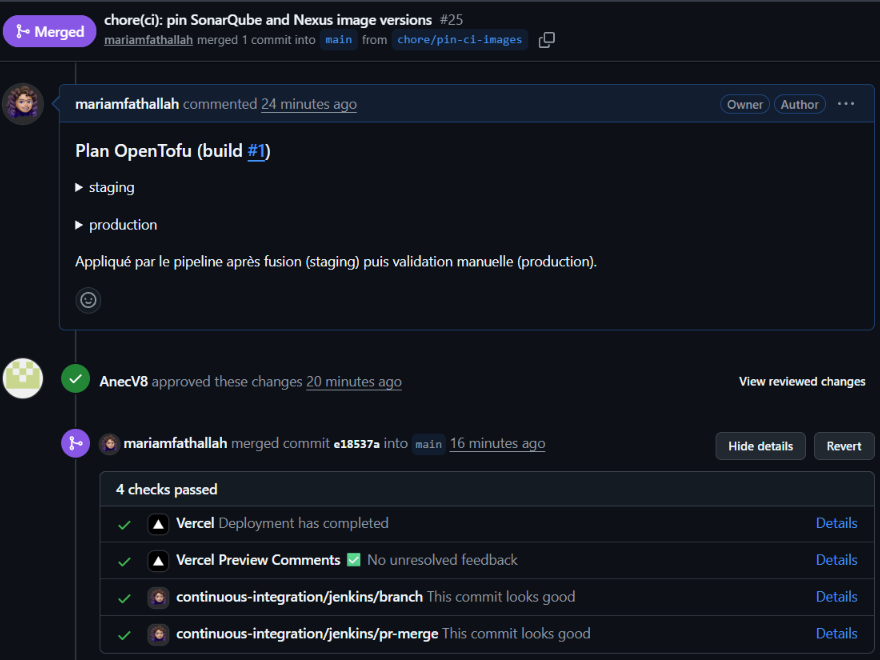
\includegraphics[width=0.85\textwidth]{pr-check.png}
  \caption{Plan OpenTofu publié sur la PR, approbation et checks Jenkins verts}
\end{figure}

Quand plusieurs commits arrivent sur la même branche, seul le dernier est construit (\texttt{disableConcurrentBuilds(abortPrevious: true)}).

L'application étant déjà en ligne avant le projet (Render et Vercel déployaient \texttt{main}), le site public a été déplacé sur une branche \texttt{live}. \texttt{main} est ainsi devenue la branche du projet : chaque fusion y est publiée, déployée en staging, puis en production après validation.
Cette migration a été fusionnée par \emph{merge commit}, seule exception à la règle du squash, pour que les tags existants restent atteignables depuis \texttt{main} et que semantic-release poursuive la numérotation.

\section{Shared Library}
La bibliothèque (\url{https://github.com/l3miage-morabitb/jenkins-shared-library}) expose trois fonctions dans son dossier \texttt{vars/}. Le nom du fichier est le nom de la fonction.

\begin{table}[H]
  \centering
  \small
  \begin{tabularx}{\textwidth}{@{}L{3.6cm}YL{1.6cm}@{}}
    \toprule
    \textbf{Fonction} & \textbf{Rôle} & \textbf{Version} \\
    \midrule
    \texttt{notifyDiscord()} & message de fin de build (statut, lien), dans \texttt{post \{ always \}} & v1.0.1 \\
    \texttt{publishToNexus()} & envoi du jar versionné dans Nexus & v1.1.0 \\
    \texttt{deployTo(env)} & déploiement via \texttt{ci/scripts/deploy.sh}, qui reste inchangé & v1.2.0 \\
    \bottomrule
  \end{tabularx}
  \caption{Fonctions de la Shared Library}
\end{table}

\textbf{Versionnage.} Ajouter une fonction fait monter le deuxième chiffre, et un tag publié n'est jamais déplacé. La version v1.0.0 contenait une fonction \texttt{notify}, renommée \texttt{notifyDiscord} en v1.0.1 : Jenkins appelait la méthode Java native \texttt{Object.notify()}, refusée par le sandbox.

\textbf{Secrets.} La bibliothèque ne contient aucun secret. Elle lit les credentials Jenkins (\texttt{nexus-creds}, \texttt{discord-webhook}), créés par JCasC à partir de \texttt{ci/.env}.

\section{Gestion des secrets}
Aucun secret n'est écrit dans le dépôt. Chaque membre les place dans un fichier \texttt{ci/.env}, exclu par le \texttt{.gitignore} ; seul le modèle \texttt{ci/.env.example}, sans valeurs, est versionné. Au démarrage, JCasC transforme ces variables en \textbf{credentials Jenkins} :

\begin{table}[H]
  \centering
  \small
  \begin{tabularx}{\textwidth}{@{}L{3.2cm}L{3.2cm}Y@{}}
    \toprule
    \textbf{Credential} & \textbf{Type} & \textbf{Utilisation} \\
    \midrule
    \texttt{sonar-token} & texte secret & analyse SonarQube (\texttt{withSonarQubeEnv}) \\
    \texttt{github-token} & utilisateur + token & lecture du dépôt, statut des PR, commentaire du plan, releases \\
    \texttt{nexus-creds} & utilisateur + mot de passe & publication et téléchargement des artefacts \\
    \texttt{discord-webhook} & texte secret & notifications de fin de build \\
    \bottomrule
  \end{tabularx}
  \caption{Credentials Jenkins créés par JCasC}
\end{table}

Le pipeline n'y accède que par \texttt{credentials()} et \texttt{withCredentials}, et Jenkins masque leur valeur dans les journaux (\texttt{****}). Le token GitHub est un token \emph{fine-grained}, limité au seul dépôt : en lecture seule pour les membres, et avec les droits d'écriture nécessaires (statuts, commentaires, releases) pour le seul Jenkins de référence.

Les secrets des environnements (mot de passe de la base, clé JWT) suivent un autre chemin : ils sont générés par OpenTofu, conservés dans son état (volume \texttt{tf\_state}, hors Git), puis transmis à Ansible par un fichier temporaire supprimé après le déploiement, avec des tâches en \texttt{no\_log}.

\textbf{Limite.} Ces secrets d'environnement ne sont pas des credentials Jenkins : ils restent dans l'état OpenTofu. Une solution plus robuste serait un coffre-fort de secrets (Vault, par exemple) partagé par OpenTofu et Jenkins.

% =====================================================================
\chapter{Environnements et déploiement}\label{chap:deploiement}
% Staging, production, blue/green, Terraform/Ansible.

\section{Staging et production}
Staging et production sont décrits par \textbf{le même code} (\texttt{infra/terraform}) ; seules les valeurs changent, dans \texttt{environments/staging.tfvars} et \texttt{environments/production.tfvars} (nom et port). Chaque environnement est isolé :

\begin{table}[H]
  \centering
  \small
  \begin{tabularx}{\textwidth}{@{}L{4.2cm}Y@{}}
    \toprule
    \textbf{Ressource} & \textbf{Rôle} \\
    \midrule
    \texttt{tracker-<env>-net} & réseau Docker propre à l'environnement \\
    \texttt{tracker-<env>-db-data} & volume des données PostgreSQL, protégé contre la destruction (\texttt{prevent\_destroy}) \\
    \texttt{tracker-<env>-db} & PostgreSQL 16 avec vérification de santé (\texttt{pg\_isready}) \\
    Mot de passe de la base, clé JWT & générés par OpenTofu (32 et 64 caractères ; la clé JWT doit dépasser 256 bits) \\
    \texttt{tracker-<env>-proxy}, \texttt{-blue}, \texttt{-green} & proxy et application, créés par Ansible (section~\ref{sec:bluegreen}) ; seul le proxy est publié, sur le port 8082 (staging) ou 8083 (production) \\
    \bottomrule
  \end{tabularx}
  \caption{Ressources d'un environnement}
\end{table}

Chaque ressource porte les labels \texttt{project}, \texttt{environment} et \texttt{managed-by} (\texttt{opentofu} ou \texttt{ansible}), ce qui permet de voir avec \texttt{docker ps} quel outil gère quoi.

\section{Environnements as Code (OpenTofu et Ansible)}
\textbf{Répartition.} OpenTofu crée l'infrastructure durable de chaque environnement (section précédente). Ansible y installe l'application : téléchargement du jar depuis Nexus, construction de l'image, conteneurs blue/green, proxy et vérifications de santé.

\textbf{Dans le pipeline.}
\begin{itemize}
  \item \emph{Infra plan}, sur toutes les branches : \texttt{infra.sh plan} calcule le plan de staging et de production, l'enregistre (\texttt{<env>.tfplan}) et l'archive en texte (\texttt{plan-<env>.txt}). Sur une pull request, il est publié en commentaire : le relecteur voit l'effet d'un changement d'infrastructure avant la fusion.
  \item \emph{Deploy staging}, sur \texttt{main} : \texttt{infra.sh apply staging} applique exactement le plan enregistré plus tôt dans le même build, puis Ansible déploie la version.
  \item \emph{Deploy production} : même chose, après la validation manuelle.
\end{itemize}

\textbf{Passage des informations.} \texttt{deploy.sh} lit les outputs d'OpenTofu (réseau, nom de la base, secrets), les écrit dans un fichier temporaire lisible par son seul propriétaire, supprimé à la fin, puis lance le playbook. Les tâches qui manipulent des secrets sont en \texttt{no\_log}. Le fichier \texttt{.terraform.lock.hcl} est versionné : tout le monde utilise exactement les mêmes versions de providers.

\textbf{Vérifications.} Relancer un plan sans changement de code affiche \og No changes \fg{}. Supprimer du code le volume de données fait échouer le plan, grâce à \texttt{prevent\_destroy}.

\section{Déploiement blue/green}\label{sec:bluegreen}
Le déploiement est réalisé par le playbook \texttt{infra/ansible/bluegreen.yml} :
\begin{enumerate}
  \item lecture de la couleur active, mémorisée dans le proxy ; la nouvelle version est déployée sur la couleur \textbf{inactive}, sans toucher au trafic ;
  \item vérification de santé (\texttt{/actuator/health}) directement sur cette couleur, depuis le réseau de l'environnement ;
  \item si elle est correcte : bascule du proxy (\texttt{nginx -t} puis \texttt{nginx -s reload}, sans interruption), puis nouvelle vérification à travers le proxy ;
  \item si elle échoue : la couleur défaillante est supprimée et le proxy reste (ou revient) sur l'ancienne. C'est le \textbf{retour arrière automatique} : les utilisateurs ne voient jamais la version défaillante, et le build échoue ;
  \item l'ancienne couleur reste démarrée, pour permettre un retour arrière instantané.
\end{enumerate}

\begin{table}[H]
  \centering
  \small
  \begin{tabularx}{\textwidth}{@{}L{5cm}Y@{}}
    \toprule
    \textbf{Test} & \textbf{Résultat} \\
    \midrule
    Premier déploiement & \texttt{blue} démarré, proxy créé \\
    Nouvelle version & déployée sur \texttt{green}, bascule du proxy, \texttt{blue} conservée \\
    Même version redéployée & aucune modification (idempotence) \\
    Échec volontaire (base de données arrêtée) & santé en échec, couleur défaillante supprimée, le proxy reste sur l'ancienne couleur (\texttt{rescued=1}) \\
    Production depuis \texttt{main} & validation manuelle par \texttt{admin}, bascule de couleur, \texttt{/actuator/health} à \texttt{UP} \\
    \bottomrule
  \end{tabularx}
  \caption{Tests du déploiement blue/green}
\end{table}

\textbf{Limites.} L'ancienne couleur reste démarrée, ce qui coûte environ 400~Mo de mémoire par environnement. Surtout, les deux couleurs partagent la même base de données et les migrations Liquibase s'exécutent au démarrage de l'application : une migration non rétrocompatible (renommage ou suppression de colonne) casserait l'ancienne version pendant la bascule. L'évolution naturelle serait d'exécuter les migrations dans une étape dédiée du pipeline et d'appliquer le modèle \emph{expand/contract} : ajout, migration des données, puis suppression, sur trois releases.

\section{Idempotence et même artefact}
Le jar est construit une seule fois, publié dans Nexus sous la version \texttt{X.Y.Z-<hash>}, puis téléchargé depuis Nexus pour chaque déploiement : staging et production exécutent exactement le même artefact, celui qui a passé les tests. Chaque version est téléchargée dans son propre dossier, ce qui garantit que l'image contient bien le jar de la version annoncée.

\begin{figure}[H]
  \centering
  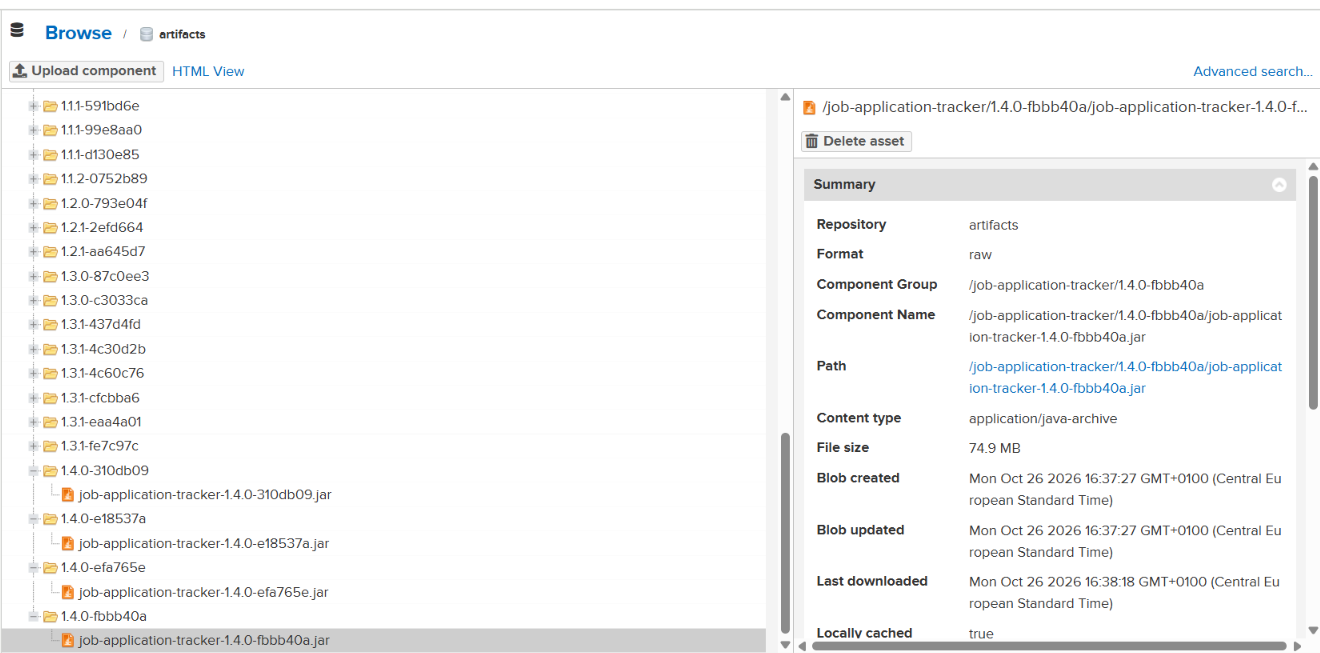
\includegraphics[width=\textwidth]{nexus.png}
  \caption{Artefacts versionnés \texttt{X.Y.Z-<hash>} dans Nexus}
\end{figure}

Relancer un déploiement ne casse rien : si la version demandée est déjà active, le playbook ne modifie rien ; de même, \texttt{tofu plan} sans changement de code affiche \og No changes \fg{}.

% =====================================================================
\chapter{Qualité}\label{chap:qualite}
% Couverture, Sonar, durée du pipeline.

\section{Tests et couverture}
Le backend est testé avec JUnit lors de \texttt{./mvnw verify}, et les résultats sont publiés dans Jenkins. JaCoCo mesure la couverture et génère \texttt{jacoco.xml}, lu par Jenkins et par SonarQube. La règle \texttt{check} fait échouer le build si la couverture des lignes passe sous le seuil de la propriété \texttt{jacoco.minimum} du \texttt{pom.xml}, fixé à \textbf{50\,\%}. Ce seuil est un plancher : le contrôle fin est assuré par la Quality Gate (80\,\% sur le nouveau code).

Sur la branche \texttt{main}, la couverture mesurée est de \textbf{87,2\,\%} pour les lignes (259 couvertes, 38 manquées), 83,3\,\% pour les branches et 88,6\,\% pour les instructions.

Les tests d'intégration lancent PostgreSQL et l'application avec \texttt{docker-compose.test.yml}. Le script \texttt{integration-test.sh} attend que \texttt{/actuator/health} réponde \texttt{UP}, puis vérifie \texttt{register} (code 201) et \texttt{login} (code 200 avec un jeton). Chaque exécuteur utilise son propre nom de projet Docker et un port choisi par Docker, donc des builds simultanés ne se gênent pas. Les conteneurs sont supprimés dans \texttt{post \{ always \}}, même en cas d'échec, et un \texttt{.dockerignore} réduit le contexte de construction.

\section{SonarQube et Quality Gate}
L'analyse SonarQube est suivie d'une Quality Gate bloquante (étape \texttt{waitForQualityGate} avec \texttt{abortPipeline: true}, délai de 5 minutes). La gate utilisée est \emph{Sonar way}, qui suit la méthode \emph{Clean as You Code} et porte sur le nouveau code :
\begin{itemize}
  \item couverture par les tests d'au moins 80\,\% ;
  \item lignes dupliquées : 3\,\% au plus ;
  \item notes A en fiabilité, sécurité et maintenabilité ;
  \item 100\,\% des \emph{security hotspots} relus.
\end{itemize}
SonarQube prévient Jenkins par un webhook (\texttt{bootstrap-sonar.sh}) ; sans lui, le build attend indéfiniment. Si la gate est rouge, rien n'est publié ni déployé.

\section{Durée du pipeline}
Avec toute la chaîne en place, un build de pull request prenait environ 5~min~30. L'analyse des étapes a montré que SonarQube, l'attente de la Quality Gate et les tests d'intégration s'exécutaient l'un après l'autre (94 à 186~s), alors qu'ils sont indépendants. Ils ont été placés en parallèle, avec \texttt{failFast} : le premier échec arrête l'autre branche.

\begin{table}[H]
  \centering
  \small
  \begin{tabular}{@{}lcc@{}}
    \toprule
    \textbf{Mesure} & \textbf{Avant} & \textbf{Après} \\
    \midrule
    SonarQube + Quality Gate + tests d'intégration & 94 à 186~s & environ 65~s \\
    Build complet d'une pull request & environ 5~min~30 & environ 3~min \\
    Build de \texttt{main} jusqu'au staging & 4,2~min & 2,7~min \\
    \bottomrule
  \end{tabular}
  \caption{Durée du pipeline avant et après la parallélisation}
\end{table}

\textbf{Fiabilité.} Certains builds échouaient pour des raisons étrangères au code : tests frontend en timeout, agent hors ligne, Docker ne répondant plus. Deux causes ont été mesurées et corrigées :
\begin{itemize}
  \item \textbf{la mémoire} : Nexus occupait environ 2~Go et les conteneurs Java de l'application n'avaient pas de limite. Les plafonds mémoire de la JVM ramènent Nexus à environ 1~Go ;
  \item \textbf{le disque} : l'agent ne dispose que de 3,9~Go, dont 3,1~Go occupés par les workspaces et les jar de toutes les versions. Seul le jar du build est désormais archivé et le workspace est supprimé en fin de build (\texttt{deleteDir()}) : il reste 3,5~Go libres.
\end{itemize}

\textbf{Limites connues.}
\begin{itemize}
  \item La publication du plan sur la PR nécessite un token GitHub en écriture ; avec un token en lecture seule, l'étape échoue. Le correctif identifié consiste à rendre ce commentaire non bloquant, le plan restant disponible en artefact.
  \item Dans \texttt{infra.sh}, le \texttt{tee} masque le code de retour de \texttt{tofu plan} : une erreur de plan n'est détectée qu'à l'étape \texttt{apply}. Correctif identifié : \texttt{set -o pipefail}.
\end{itemize}

% =====================================================================
\chapter{Métriques DORA}\label{chap:dora}
% Courbes, analyse, limites.

Les quatre métriques DORA du projet sont calculées automatiquement à partir de l'historique Jenkins et Git, sans aucune saisie manuelle, et suivies dans Grafana sur toute la durée du projet.

\section{Chaîne de mesure}
Prometheus va chercher les métriques auprès de Jenkins (plugin \texttt{prometheus}), de l'application en staging et en production (\texttt{/actuator/prometheus}) et de l'exporter DORA. Grafana les affiche dans deux tableaux de bord : une vue d'ensemble et le tableau de bord DORA. L'exporter (\texttt{ci/dora-exporter}) est la seule pièce écrite pour le module : il lit l'historique Jenkins chaque minute, calcule les quatre métriques et mémorise chaque build dans le volume \texttt{dora\_data}.

\begin{figure}[H]
  \centering
  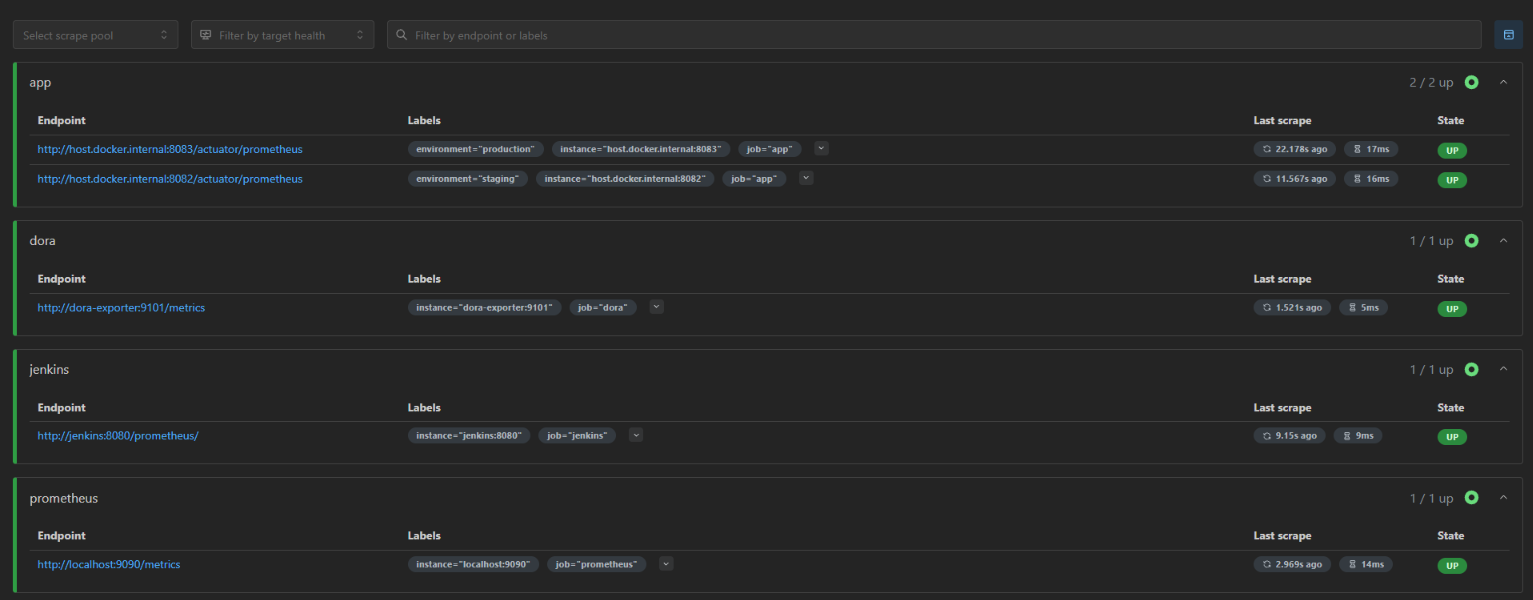
\includegraphics[width=\textwidth]{prometheus-targets.png}
  \caption{Cibles collectées par Prometheus : application (staging et production), exporter DORA, Jenkins}
\end{figure}

% \begin{figure}[H]
%   \centering
%   \includegraphics[width=\textwidth]{dora-architecture.png}
%   \caption{Chaîne de mesure des métriques DORA}
% \end{figure}

\section{Définitions et calculs}
Un déploiement est l'exécution du stage \emph{Deploy production} d'un build de la branche qui déploie. Il réussit si ce stage finit en succès, et échoue s'il finit en échec. Une validation refusée ou expirée n'est pas un déploiement.

\begin{table}[H]
  \centering
  \small
  \begin{tabularx}{\textwidth}{@{}L{3cm}YL{2.6cm}@{}}
    \toprule
    \textbf{Métrique} & \textbf{Calcul} & \textbf{Niveau élite} \\
    \midrule
    Fréquence de déploiement & déploiements réussis divisés par le nombre de jours de la période & au moins 1 par jour \\
    \addlinespace
    Délai de livraison & fin du déploiement réussi moins l'heure de chaque commit livré, puis médiane & moins d'un jour \\
    \addlinespace
    Taux d'échec des changements & déploiements échoués divisés par tous les déploiements & 0 à 15\,\% \\
    \addlinespace
    Temps de rétablissement & du premier déploiement échoué d'une série au déploiement réussi suivant, puis médiane & moins d'une heure \\
    \bottomrule
  \end{tabularx}
  \caption{Définition des métriques DORA}
\end{table}

Trois règles précisent ces calculs :
\begin{itemize}
  \item \textbf{Commits livrés} : un commit construit sans être déployé est rattaché au déploiement réussi suivant. Son délai court donc jusqu'à sa vraie mise en production.
  \item \textbf{Heure d'un commit} : elle vient des \emph{changeSets} de Jenkins. Pour le premier build d'une branche, l'exporter la lit dans l'API GitHub.
  \item \textbf{Retour arrière automatique} : si le blue/green détecte une version défaillante, il rebascule et le stage échoue. Ce cas compte comme un échec.
\end{itemize}

Chaque métrique est calculée sur trois périodes : 7 jours, 30 jours et toute la durée du projet.

\section{Résultats}
Les valeurs ci-dessous viennent du tableau de bord DORA du Jenkins de référence, relevées le 1\textsuperscript{er} novembre 2026. Elles couvrent environ une semaine de déploiements, d'abord sur la branche \texttt{feature/ci-jenkins} puis sur \texttt{main}, qui déploie depuis le 26 octobre.

\begin{table}[H]
  \centering
  \begin{tabular}{@{}lcc@{}}
    \toprule
    \textbf{Métrique} & \textbf{Valeur mesurée} & \textbf{Niveau DORA} \\
    \midrule
    Fréquence de déploiement & 1,99 par jour & élite \\
    Délai de livraison (médiane) & 1,5 heure & élite \\
    Taux d'échec des changements & 13\,\% (2 sur 16) & élite \\
    Temps de rétablissement (médiane) & 14,7 minutes & élite \\
    \midrule
    Déploiements réussis / échoués & 14 / 2 & \textendash \\
    \bottomrule
  \end{tabular}
  \caption{Métriques DORA mesurées}
\end{table}

\begin{figure}[H]
  \centering
  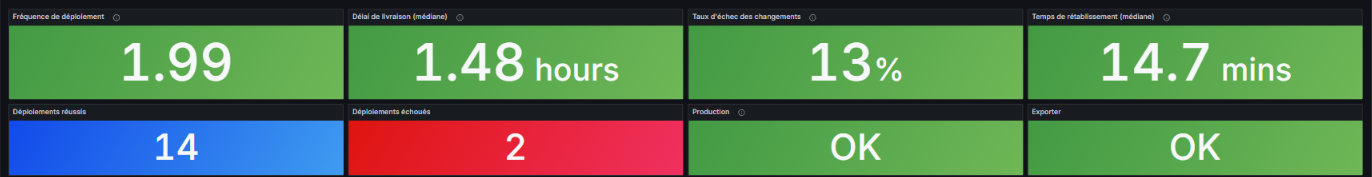
\includegraphics[width=\textwidth]{dora-dashboard.png}
  \caption{Tableau de bord DORA dans Grafana (Jenkins de référence)}
\end{figure}

\section{Analyse}
Les quatre métriques se situent au niveau \enquote{élite} des repères DORA. Ce résultat est à lire avec prudence vu la taille de l'échantillon (voir les limites).

\textbf{Vitesse.} Avec 14 mises en production réussies en une semaine, l'équipe déploie environ deux fois par jour. Chaque pull request fusionnée part en production le jour même. Le délai médian d'une heure et demie entre un commit et sa mise en production est surtout fait d'attente humaine : relecture de la pull request (une approbation obligatoire) et clic de validation avant la production. Le pipeline lui-même dure moins de 10 minutes.

\textbf{Stabilité.} Le tableau de bord compte deux échecs sur 16, chacun rétabli en un quart d'heure environ (14,7 minutes en médiane). En analysant ces deux builds, nous avons constaté qu'aucun ne correspond à une mise en production ratée :
\begin{itemize}
  \item \textbf{après la fusion de la PR \#14}, l'agent Jenkins a manqué de mémoire pendant les tests du frontend : il s'est déconnecté et les tests Vitest ont expiré. Le stage \emph{Lint \& tests} a échoué et toutes les étapes suivantes ont été sautées. Le build relancé 13,5 minutes plus tard a réussi. Pour éviter que cela se reproduise, la mémoire de Nexus et des conteneurs de l'application a été limitée (PR \#17) ;
  \item \textbf{après la fusion de la PR du README}, c'est le déploiement en staging qui a échoué. Les conteneurs de staging et de production étaient arrêtés depuis plusieurs jours : Ansible n'a pas trouvé de couleur active, a recréé le proxy nginx et l'a rechargé avant qu'il ait fini de démarrer (\emph{invalid PID number}). Le build s'est arrêté avant toute bascule et la production a été sautée. Il a été relancé avec succès ; le correctif identifié consiste à réessayer le rechargement de nginx quelques secondes plus tard.
\end{itemize}

Dans les deux cas, aucune version défaillante n'a été mise en ligne. Mais Jenkins marque comme échoués les stages sautés après une erreur, et l'exporter a donc compté ces deux builds comme des déploiements échoués. Au sens strict de DORA, qui ne retient que les échecs de la mise en production elle-même, le taux d'échec réel de la période est de 0\,\%, et le temps de rétablissement n'a pas pu être mesuré faute d'incident en production. Les valeurs affichées décrivent plutôt la stabilité de la chaîne de livraison, ce qui reste une information utile : les deux pannes venaient de l'environnement local, pas du code, et ont été résolues en un quart d'heure.

\section{Limites}
\begin{itemize}
  \item \textbf{Petit échantillon} : une douzaine de déploiements sur une semaine. Un seul échec suffit à faire varier fortement le taux d'échec.
  \item \textbf{Période partielle} : Jenkins ne garde que les 20 derniers builds de chaque branche. Quand l'exporter a été mis en service le 26 octobre, les builds plus anciens avaient déjà été supprimés : la mesure ne couvre donc que la dernière semaine du projet.
  \item \textbf{Échec avant la production} : un build qui échoue avant le déploiement est compté comme un déploiement échoué, car Jenkins marque les stages sautés comme échoués. C'est le cas des deux échecs mesurés (voir l'analyse).
  \item \textbf{Une seule instance fait foi} : seul le Jenkins de référence a l'historique complet ; les Jenkins des autres membres ne voient que leurs propres builds.
  \item \textbf{Production locale} : staging et production tournent sur un poste de développement. Un échec peut venir de la machine (mise en veille, mémoire) et non du code.
  \item \textbf{Échec = échec du déploiement} : un bug découvert après une mise en production réussie n'est pas compté.
  \item \textbf{Validation manuelle} : elle allonge le délai de livraison selon la disponibilité de l'équipe.
  \item \textbf{Historique dépendant d'un volume} : supprimer le volume \texttt{dora\_data} efface les déploiements que Jenkins ne garde plus.
\end{itemize}

% =====================================================================
\chapter{Difficultés rencontrées et solutions}

\begin{table}[H]
  \centering
  \small
  \begin{tabularx}{\textwidth}{@{}YY@{}}
    \toprule
    \textbf{Difficulté} & \textbf{Solution} \\
    \midrule
    La Quality Gate attendait indéfiniment & ajout du webhook SonarQube vers Jenkins (\texttt{bootstrap-sonar.sh}) \\
    Scripts en échec dans les conteneurs à cause des fins de ligne Windows & fins de ligne LF imposées par \texttt{.gitattributes} \\
    Docker Desktop bloqué par manque de mémoire & 8 Go réservés à WSL, mémoire de Nexus et de l'application limitée \\
    \addlinespace
    Webhook reçu mais refusé (HTTP 405) : la version 5 de \texttt{smee-client} retire le \texttt{/} final de l'URL & version épinglée \texttt{smee-client@2.0.4} \\
    \addlinespace
    \texttt{ci/.env.example} absent du dépôt, exclu par la règle \texttt{.env.*} & exception \texttt{!ci/.env.example} dans le \texttt{.gitignore} \\
    \addlinespace
    commitlint 21 et semantic-release 24 exigent deux versions incompatibles d'une même dépendance & commitlint 20, lock régénéré sur l'agent et vérifié par \texttt{npm ci} \\
    \addlinespace
    Notes de version en double après une fusion par \emph{merge commit} & fusion en \emph{squash} uniquement sur \texttt{main} \\
    \addlinespace
    Agent hors ligne, faute de disque & archivage du seul jar du build et \texttt{deleteDir()} en fin de build \\
    \addlinespace
    \texttt{main} déployait déjà le site public : impossible d'y déployer la chaîne Jenkins & site public déplacé sur une branche \texttt{live}, puis \texttt{main} devenue branche de déploiement \\
    \addlinespace
    Secret Discord créé à la main, absent chez les collègues & déclaré dans \texttt{casc.yaml} et \texttt{docker-compose.yml}, comme \texttt{sonar-token} \\
    Fonction \texttt{notify} refusée par le sandbox (\texttt{Object.notify}) & renommée \texttt{notifyDiscord} (tag v1.0.1) \\
    Tests d'intégration en conflit entre builds parallèles & nom de projet par exécuteur et port choisi par Docker \\
    Contexte de construction Docker trop lourd & \texttt{.dockerignore} ciblé \\
    Envoi dans Nexus refusé (403) & Jenkins recréé pour relire \texttt{ci/.env} \\
    \addlinespace
    Les conteneurs lancés par les builds (Docker de l'hôte) ne voyaient pas les fichiers du workspace de l'agent & workspace monté au même chemin (\texttt{/opt/jenkins-agent}) côté hôte et côté agent \\
    \addlinespace
    Clé JWT générée trop courte, refusée par l'application & clé de 64 caractères (plus de 256 bits) \\
    \addlinespace
    Image construite avec le jar d'une ancienne version (le téléchargement ne remplace pas un fichier existant) & un dossier de téléchargement par version (\#16) \\
    \bottomrule
  \end{tabularx}
  \caption{Difficultés et solutions}
\end{table}

% =====================================================================
\chapter{Répartition du travail}

\begin{table}[H]
  \centering
  \begin{tabularx}{\textwidth}{@{}lY@{}}
    \toprule
    \textbf{Membre} & \textbf{Réalisations} \\
    \midrule
    Basma MORABIT & Shared Library versionnée par tag, tests d'intégration, module Qualité \\
    Bastien LIEVRE & mise en place de l'outillage (Docker Compose, JCasC, agent) et du premier pipeline, module Environnements as Code (OpenTofu, Ansible) \\
    Siham AIDROUS & Module Observabilité et DORA : Prometheus, Grafana, exporter DORA \\
    Mariam FATHALLAH & liaison GitHub, webhook, statut des PR, modules Releases et Blue/green, optimisation et fiabilité du pipeline, migration de la branche de déploiement \\
    \bottomrule
  \end{tabularx}
  \caption{Répartition du travail}
\end{table}

Chaque tâche a été réalisée sur sa propre branche (\texttt{module/<nom>}, \texttt{fix/\ldots}, \texttt{docs/\ldots}), puis proposée par pull request vers \texttt{main}. Une PR ne peut être fusionnée qu'après un build Jenkins vert et la relecture d'un autre membre ; la fusion se fait en \emph{squash}, avec un message au format Conventional Commits. La documentation d'équipe (\texttt{docs/EQUIPE.md}) décrit ce workflow, la répartition des tâches et les problèmes déjà rencontrés, ce qui a permis à chacun de faire tourner la chaîne sur son propre poste.

% =====================================================================
\chapter*{Conclusion}
\addcontentsline{toc}{chapter}{Conclusion}

\section*{Bilan}
L'objectif du projet est atteint : la partie commune et les cinq modules choisis fonctionnent, dont les deux de niveau 3. Chaque commit sur \texttt{main} est construit, testé, analysé, versionné, publié dans Nexus, puis déployé en staging et, après validation, en production, sans aucune action manuelle en dehors de ce clic de validation. Toute la chaîne est décrite dans le dépôt : la plateforme, la configuration de Jenkins, le pipeline et les environnements se recréent à partir du code et d'un fichier \texttt{.env}.

Quelques chiffres résument le résultat :
\begin{itemize}
  \item un build complet d'une pull request dure environ 3 minutes, contre 5 min 30 avant la parallélisation ;
  \item la couverture des lignes atteint 87,2\,\%, et la Quality Gate bloque tout code qui ne respecte pas ses conditions ;
  \item neuf versions ont été calculées et publiées automatiquement par semantic-release ;
  \item les quatre métriques DORA mesurées se situent au niveau \enquote{élite}, avec environ deux mises en production par jour.
\end{itemize}

\section*{Ce que le projet nous a appris}
Le premier enseignement est qu'une chaîne CI/CD se construit par étapes et se vérifie en continu. Plusieurs problèmes ne sont apparus qu'à l'usage : la mémoire de Docker Desktop, le disque de l'agent, les fins de ligne Windows, ou une version de \texttt{smee-client} qui modifiait l'URL du webhook. Chacun a été corrigé dans le code et documenté, pour ne pas se reproduire chez les autres membres.

Le deuxième concerne le travail en équipe. Les règles appliquées au code (une branche par tâche, une pull request relue par un autre membre, un build vert obligatoire) ont évité de casser la branche principale, et la relecture croisée a obligé chacun à comprendre des parties qu'il n'avait pas écrites.

Enfin, mesurer la chaîne nous a appris à interpréter les chiffres avec prudence. L'analyse des métriques DORA a montré que les deux échecs comptés par la mesure n'étaient pas des mises en production ratées, mais des builds arrêtés avant la production. Un indicateur n'a de valeur que si l'on sait exactement ce qu'il compte.

\section*{Améliorations possibles}
\begin{itemize}
  \item \textbf{Environnements dans le cloud} : remplacer le provider Docker d'OpenTofu par celui d'un hébergeur, la structure du code restant la même, pour ne plus dépendre d'un poste de développement.
  \item \textbf{Migrations de base de données} : les exécuter dans une étape dédiée du pipeline, selon le modèle \emph{expand/contract}, pour rendre le blue/green sûr même en cas de changement de schéma.
  \item \textbf{Secrets} : réunir les secrets de Jenkins et ceux des environnements dans un coffre-fort comme Vault.
  \item \textbf{Mesure DORA} : ne compter comme échec que les erreurs du stage de production, et relier les incidents découverts après une mise en production à la version concernée.
  \item \textbf{Robustesse} : rendre non bloquante la publication du plan sur les pull requests, ajouter \texttt{set -o pipefail} au script d'infrastructure et réessayer le rechargement de nginx quand le proxy vient d'être recréé, trois correctifs déjà identifiés.
\end{itemize}

En quelques semaines, nous sommes passés d'une application déployée à la main à une chaîne qui livre en production plusieurs fois par jour, de façon traçable et mesurée. C'est la base sur laquelle ces améliorations pourraient être construites.

\end{document}
